\documentclass{beamer}

% Required packages
\usepackage{xcolor}
\usepackage{tikz}
\usepackage{amsmath}
\usepackage{listings}

% Define custom colors
\definecolor{ds9blue}{RGB}{25,25,112}
\definecolor{ds9gold}{RGB}{218,165,32}
\definecolor{ds9grey}{RGB}{105,105,105}
\definecolor{ds9red}{RGB}{178,34,34}

% Theme configuration
\usetheme{Madrid}
\usecolortheme{whale}
\setbeamercolor{structure}{fg=ds9blue}
\setbeamercolor{alerted text}{fg=ds9red}
\setbeamercolor{example text}{fg=ds9gold}

% Title page configuration
\title[Prompt Engineering]{Physics 11-12: Prompt Engineering Guide}
\subtitle{Effective AI Communication for Physics Students}
\author[Mr. Gullo]{Mr. Gullo}
\date[Feb 2025]{February, 2025}
\institute[Physics Dept.]{Department of Physics}

\begin{document}

% Title page
\frame{\titlepage}

% Table of contents
\begin{frame}
\frametitle{Overview}
\tableofcontents
\end{frame}

% Core Principles
\section{Core Principles}
\frame{\sectionpage}
\begin{frame}
\frametitle{Core Principles}
This guide combines principles from Google's 10 Hour Prompting Essentials and Anthropic's prompting framework:

\begin{block}{Five-Step Framework}
\begin{enumerate}
\item \textbf{Task:} Clearly define what you want the AI to do
\item \textbf{Context:} Provide relevant background information
\item \textbf{References:} Incorporate examples to clarify your needs
\item \textbf{Evaluate:} Assess the AI's output
\item \textbf{Iterate:} Refine your prompt based on evaluation
\end{enumerate}
\end{block}
\end{frame}

\begin{frame}
\frametitle{Prompting Techniques}
\begin{block}{Key Techniques from Emergent Capabilities}
\begin{itemize}
\item \textbf{Role Setting:} Encourage the AI to take on the characteristics of an expert in the chosen task
\item \textbf{Chain of Thought Reasoning:} Prompt the LLM to explicitly state its reasoning process step by step before answering to allow for more thorough and well-reasoned responses to complex queries
\end{itemize}
\end{block}
\end{frame}

\section{Physics-Specific Examples}
\frame{\sectionpage}
% Quantum Mechanics Example - Edited
\begin{frame}
\frametitle{Quantum Mechanics Example}
\begin{block}{Weak vs. Optimized Prompts}
\textbf{Weak Prompt:} 
\begin{itemize}
\item "Explain quantum mechanics."
\end{itemize}

\textbf{Optimized Prompt:}
\begin{itemize}
\item "You are a high school physics teacher. Explain wave-particle duality using the double-slit experiment and photoelectric effect. Include diagrams that would help 11th-grade students understand these concepts. Use everyday analogies where possible."
\end{itemize}
\end{block}

\begin{alertblock}{Breakdown}
\begin{itemize}
\item Task: Explain wave-particle duality with specific examples
\item Context: For 11th-grade students
\item References: Double-slit experiment and photoelectric effect
\end{itemize}
\end{alertblock}
\end{frame}

% Thermodynamics Example - Edited
\begin{frame}
\frametitle{Thermodynamics Example}
\begin{block}{Weak vs. Optimized Prompts}
\textbf{Weak Prompt:}
\begin{itemize}
\item "What is entropy?"
\end{itemize}

\textbf{Optimized Prompt:}
\begin{itemize}
\item "You are a high school physics teacher. Explain entropy as energy dispersal using everyday examples like ice melting in a drink. Include a simple equation for entropy change and how it relates to the second law of thermodynamics. Keep math at an algebra level."
\end{itemize}
\end{block}

\begin{alertblock}{Breakdown}
\begin{itemize}
\item Task: Explain entropy with everyday examples
\item Context: High school algebra-level math
\item References: Ice melting example, second law connection
\end{itemize}
\end{alertblock}
\end{frame}

% Electromagnetism Example - Edited
\begin{frame}
\frametitle{Electromagnetism Example}
\begin{block}{Weak vs. Optimized Prompts}
\textbf{Weak Prompt:}
\begin{itemize}
\item "Explain Maxwell's equations."
\end{itemize}

\textbf{Optimized Prompt:}
\begin{itemize}
\item "You are a high school physics teacher. Explain the relationship between electricity and magnetism through Faraday's law of induction. Describe how a simple electric generator works based on this principle. Include a diagram suitable for 12th-grade students."
\end{itemize}
\end{block}

\begin{alertblock}{Breakdown}
\begin{itemize}
\item Task: Explain electricity-magnetism relationship
\item Context: 12th-grade level
\item References: Faraday's law, electric generator example
\end{itemize}
\end{alertblock}
\end{frame}

% Solving Derivations - Edited
\begin{frame}
\frametitle{Solving Derivations}
\begin{exampleblock}{Example Prompt}
"You are a high school physics teacher. Derive the equations for projectile motion starting from the basic kinematic equations. Show each step clearly and include a practical example of a basketball shot. Assume the student knows basic algebra and trigonometry. Think step-by-step."
\end{exampleblock}

\begin{alertblock}{Breakdown}
\begin{itemize}
\item Task: Derive projectile motion equations
\item Context: High school algebra and trigonometry
\item References: Basketball shot example
\end{itemize}
\end{alertblock}
\end{frame}

% Designing Experiments - Edited
\begin{frame}
\frametitle{Designing Experiments}
\begin{exampleblock}{Example Prompt}
"You are a high school physics teacher. Design an experiment to measure the acceleration due to gravity using a pendulum. Suggest a detailed setup suitable for a high school lab, including equipment, procedure, and expected calculations. Include a discussion of potential errors and how to minimize them."
\end{exampleblock}

\begin{alertblock}{Breakdown}
\begin{itemize}
\item Task: Design a pendulum experiment for gravity
\item Context: High school lab setting
\item References: Equipment list, error analysis
\end{itemize}
\end{alertblock}
\end{frame}

% Explaining Concepts - Edited
\begin{frame}
\frametitle{Explaining Concepts}
\begin{exampleblock}{Example Prompt}
"You are a high school physics teacher. Explain conservation of momentum to 11th-grade students. Use examples from vehicle collisions and lab demonstrations. Address common misconceptions and explain how this principle applies in everyday life. Think step-by-step."
\end{exampleblock}

\begin{alertblock}{Breakdown}
\begin{itemize}
\item Task: Explain conservation of momentum
\item Context: 11th-grade level
\item References: Vehicle collisions, lab demonstrations
\end{itemize}
\end{alertblock}
\end{frame}

\section{Safety and Ethics}
\frame{\sectionpage}
\begin{frame}
\frametitle{Academic Integrity and Safety Guidelines}
\begin{block}{Academic Integrity}
\begin{itemize}
\item Do not use AI to complete assignments or exams without understanding the underlying concepts
\item Use it as a tool to deepen understanding and check work
\end{itemize}
\end{block}

\begin{alertblock}{Common Pitfalls}
\begin{itemize}
\item Avoid oversimplification: AI can provide oversimplified answers that lack nuance
\item Always critically evaluate the AI's output
\item Consult multiple sources to ensure accuracy
\end{itemize}
\end{alertblock}
\end{frame}

\section{LLM Selection for Physics}
\frame{\sectionpage}

\begin{frame}
\frametitle{Choosing the Right LLM for Physics Tasks}

\begin{block}{Best Practices}
\begin{itemize}
\item Match LLM strengths to specific tasks
\item Consider using multiple models for different use cases
\item Verify outputs against known physics principles
\item Use benchmarks as guidelines, not absolute measures
\end{itemize}
\end{block}
\begin{figure}
    \centering
    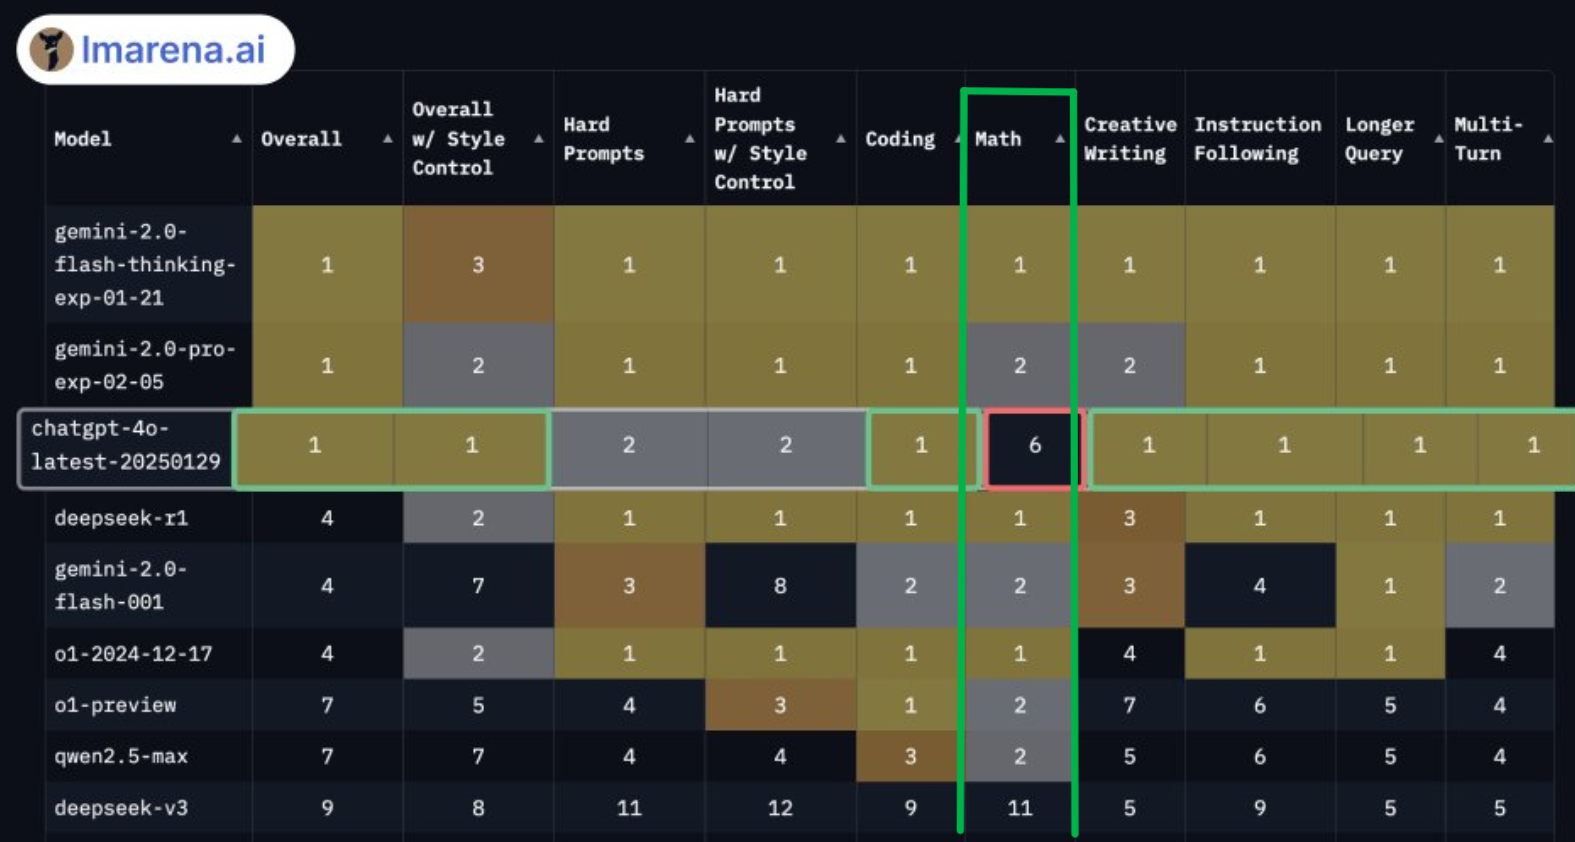
\includegraphics[width=1\linewidth]{benchmarks.png}
\end{figure}
\end{frame}



\section{OpenStax-Gemini Partnership (Depricated?)}
\frame{\sectionpage}

\begin{frame}
\frametitle{OpenStax Integration with Google Gemini}

\begin{block}{Accessing Trustworthy Educational Content}
\begin{itemize}
\item OpenStax has partnered with Google to integrate their library with Gemini (August 2024)
\item 70+ openly licensed, peer-reviewed textbooks now accessible via Gemini
\item Available to Gemini users 18+ in the United States
\end{itemize}
\end{block}

\begin{exampleblock}{How to Access}
\begin{center}
\texttt{@OpenStax explain the concept of supply and demand?}
\end{center}
\end{exampleblock}

\begin{alertblock}{Benefits for Physics Students}
\begin{itemize}
\item Accurate, attribution-based responses for physics concepts
\item Integration with other Gemini AI capabilities
\item Ensures academic integrity while using AI tools
\end{itemize}
\end{alertblock}
\end{frame}

\begin{frame}
\frametitle{OpenStax and AI in Education}

\begin{columns}
\column{0.5\textwidth}
\begin{block}{Core Principles}
\begin{itemize}
\item Accuracy in educational content
\item Proper attribution to sources
\item Accessibility for all learners
\item Preservation of academic integrity
\end{itemize}
\end{block}

\column{0.5\textwidth}
\begin{alertblock}{Quote}
\small ``OpenStax and Google share a unified, responsible vision for the use of AI in education. We believe content provided through AI learning tools should be accurate and inclusive.''
\begin{flushright}
\scriptsize — Professor Richard G. Baraniuk,\\founder and director of OpenStax
\end{flushright}
\end{alertblock}
\end{columns}

\vspace{0.5cm}
\begin{block}{Impact for Physics Education}
\begin{itemize}
\item Access to high-quality physics textbooks through a conversational AI
\item Support for challenging physics concepts with trusted content
\item Democratizing access to educational resources
\end{itemize}
\end{block}
\end{frame}

\section{Using Anthropic's Console}
\frame{\sectionpage}

\begin{frame}
\frametitle{Using Anthropic's Console}
\begin{figure}
    \centering
    \includegraphics[width=1\linewidth]{anthropiconsole.png}
\end{figure}
\end{frame}

\begin{frame}
\frametitle{Available Advanced Tools}
\begin{enumerate}
\item \textbf{Prompt Optimizer}
\begin{itemize}
\item Utilize the prompt optimizer to refine prompts
\item Improve performance through suggested modifications
\end{itemize}

\item \textbf{Prompt Generator}
\begin{itemize}
\item Create production-ready prompt templates
\item Describe desired task and output format
\end{itemize}

\item \textbf{Test Cases}
\begin{itemize}
\item Generate automatic test cases
\item Compare outputs side by side
\item Facilitate rapid iteration and refinement
\end{itemize}
\end{enumerate}
\end{frame}
\section{XML Tags in Prompting}
\frame{\sectionpage}

\begin{frame}
\frametitle{Using XML Tags in Prompts (!Advanced!)}

\begin{block}{Purpose of XML Tags}
\begin{itemize}
\item Structure content in a clear, machine-readable format
\item Separate different types of information
\item Make prompts more organized and specific
\end{itemize}
\end{block}

\begin{exampleblock}{Common XML Tag Examples}
\begin{itemize}
\item \texttt{<task>}Define specific instructions\texttt{</task>}
\item \texttt{<context>}Provide background information\texttt{</context>}
\item \texttt{<example>}Show sample content\texttt{</example>}
\item \texttt{<output>}Specify desired format\texttt{</output>}
\end{itemize}
\end{exampleblock}

\end{frame}

\section{Additional LLM Tools}
\frame{\sectionpage}

\begin{frame}
\frametitle{Exploring Other LLM Research Tools}

\begin{block}{Alternative AI Research Assistants}
\begin{description}
\item[Perplexity] \hfill \\
   \begin{itemize}
   \item Real-time search integration
   \item Academic paper analysis
   \item Direct citation capabilities 
   \item Built-in fact-checking
   \end{itemize}
   
\item[Google or OpenAi: Deep Research] \hfill \\
   \begin{itemize}
   \item Specialized for academic research
   \item Literature review assistance
   \item Paper summarization
   \item Research methodology guidance
   \end{itemize}
\end{description}
\end{block}


\end{frame}


\begin{frame}
\frametitle{Summary}
\begin{itemize}
\item Apply the five-step framework for effective prompts
\item Use role setting and chain of thought reasoning
\item Create detailed, context-rich prompts for physics problems
\item Maintain academic integrity while using AI tools
\item Leverage Anthropic's Console for prompt optimization
\item Always verify and cross-reference AI-generated content
\end{itemize}
\end{frame}

\section{Sources}
\frame{\sectionpage}

\begin{frame}[allowframebreaks]
\frametitle{Sources \& References}

\begin{block}{Core Resources}
\begin{itemize}
\item Google's 10 Hour Prompting Essentials Course\\
    \texttt{https://grow.google/prompting-essentials/}
\item OpenStax and Google Gemini Partnership\\
    \texttt{https://openstax.org/blog/press-release-openstax-partners-googles-gemini-apps}
\item LM Arena Chatbot Leaderboard\\
    \texttt{https://lmarena.ai/?leaderboard}
\end{itemize}
\end{block}

\begin{block}{Additional Tools \& Guides}
\begin{itemize}
\item Google Gemini for Education\\
    \texttt{https://gemini.google.com/education}
\item OpenStax Free Textbooks\\
    \texttt{https://openstax.org}
\item MIT Sloan Effective Prompts Guide\\
    \texttt{https://mitsloanedtech.mit.edu/ai/basics/effective-prompts/}
\end{itemize}
\end{block}
\end{frame}

\begin{frame}
\begin{figure}
    \centering
    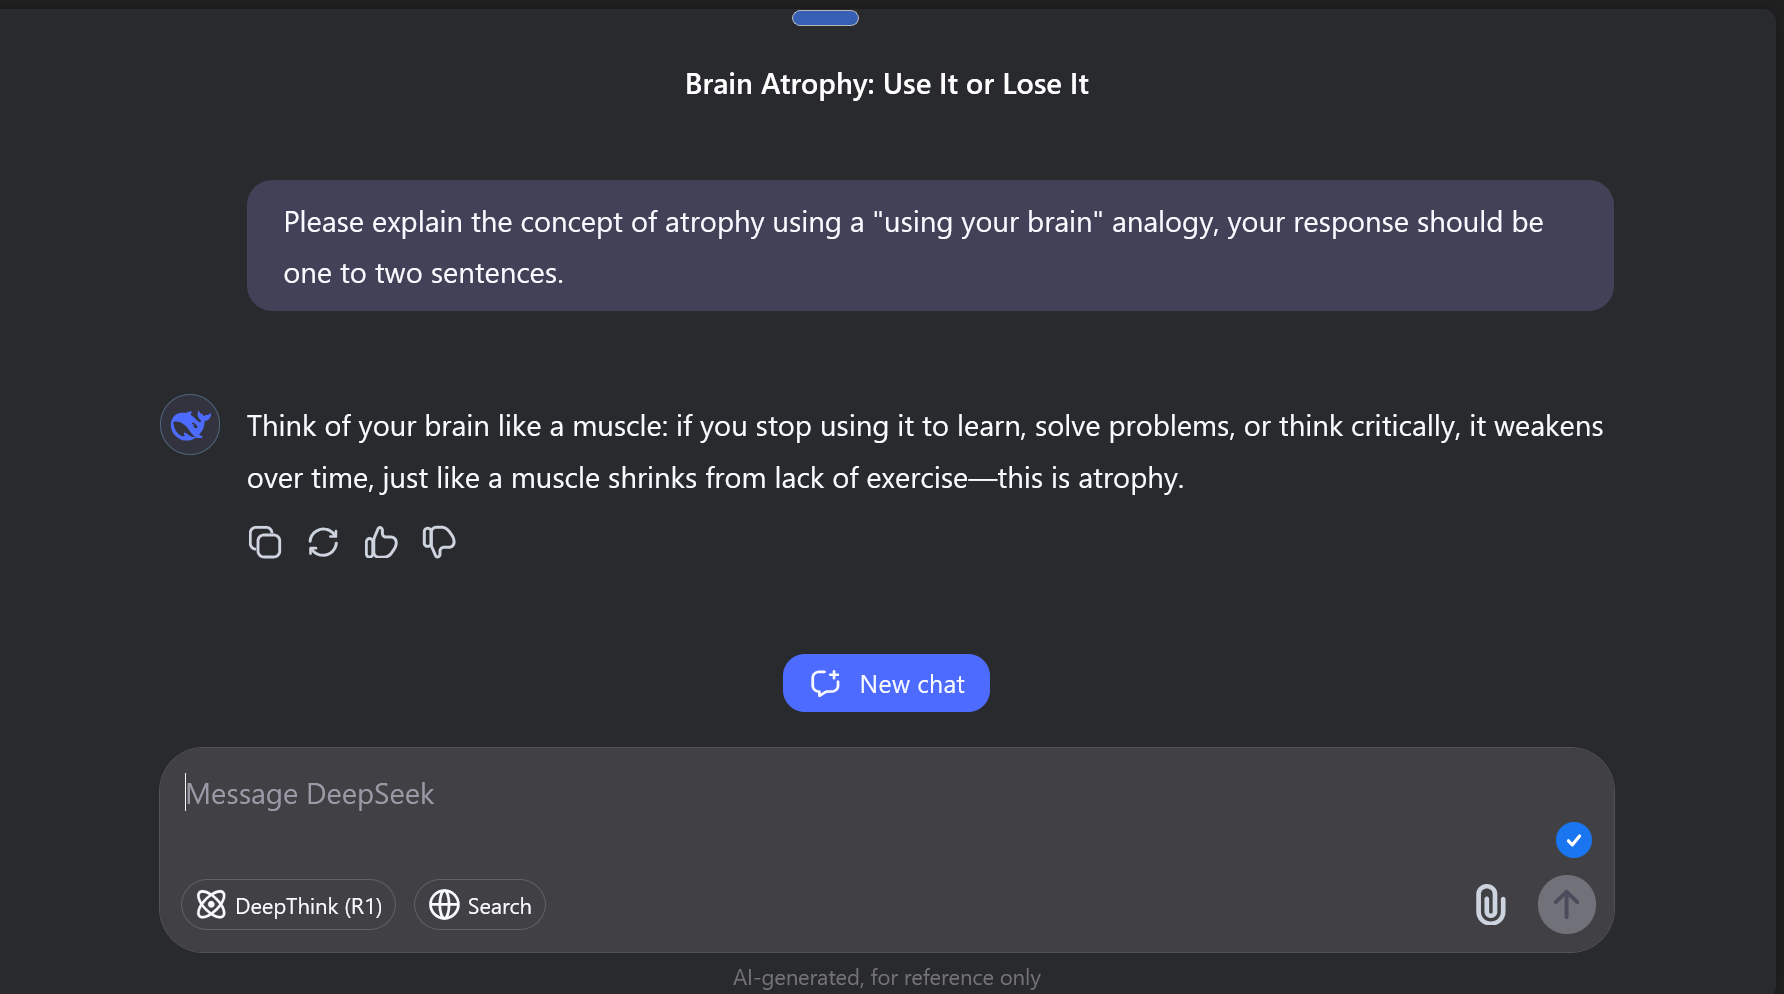
\includegraphics[width=1\linewidth]{image.png}
\end{figure}
\end{frame}
\end{document}